\section{\dssmrlong}
\subsection{General idea}
\label{sec:dssmr-idea}

Dynamic \ssmr\ (\dssmr) defines a dynamic mapping of variables to partitions.
Each variable $v$ is mapped to partition $\ppm$, meaning that $v \in \ppm$. Such
a mapping is managed by a partitioning oracle, which is implemented as a
replicated service run by a group of server processes $\ssm_0$. The oracle
service allows the mapping of variables to partitions to be retrieved or changed
during execution. In more detail, \dssmr\ distinguishes five types of commands:
$access(\omega)$ is an application command that accesses (reads or writes)
variables in set $\omega \subseteq \vvm$ (as described in
Section~\ref{sec:sysmodel}), $create(v)$ creates a new variable $v$ and
initially maps it to a partition defined by the oracle, $delete(v)$ removes $v$
from the service state,
$move(v,\ppm_s,\ppm_d)$ moves variable $v$ from partition $\ppm_s$ to partition
$\ppm_d$, and $consult(C)$ asks the oracle which variables are accessed by
command $C$, and which partition contains each of them. The reply from the
oracle to a $consult$ command is called a $prophecy$. A prophecy usually
consists of a set of tuples $\langle v, \ppm \rangle$, meaning that variable $v$
is mapped to partition $\ppm$. The other possible values for a prophecy are $ok$
and $nok$, which mean that a command can and cannot be executed, respectively.

Clients can consult the oracle to know which partitions each command should be
multicast to, based on which variables are accessed by the command. If the reply
received from the oracle tells the client that the command accesses a single
partition, the client multicasts the command to that partition. If the command
accesses variables from multiple partitions, the client first multicasts one or
more $move$ commands to the oracle and to the involved partitions, with the
intent of having all variables in the same partition. Then, the command itself
is multicast to the one partition that now holds all variables accessed by the
command. If a subsequent command accesses the same variables, it will also
access a single partition. With this scheme, the access patterns of commands
will shape the mapping of variables to partitions, reducing the number of
multi-partition commands.

\begin{figure*}
\begin{minipage}[b]{1.0\linewidth}
\centering
      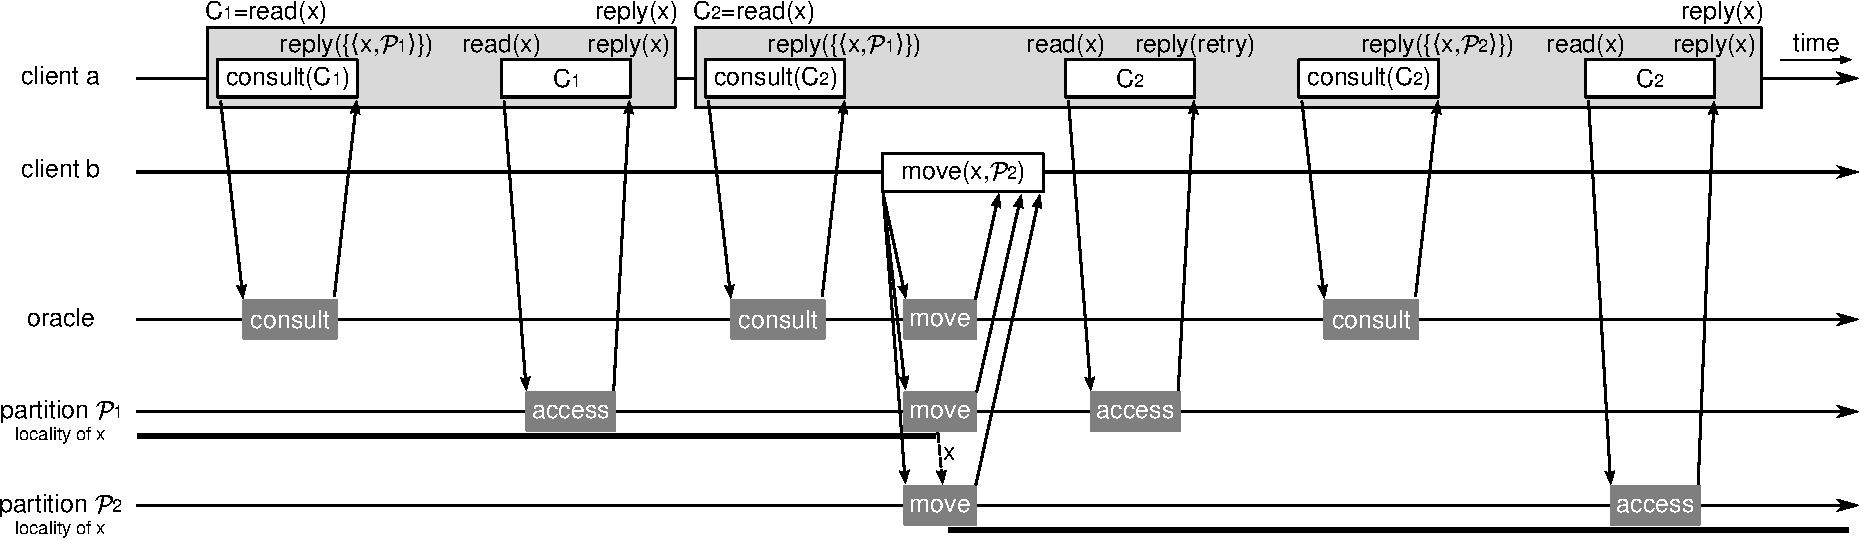
\includegraphics[width=0.8\linewidth]{figures/dssmr-detail}
\end{minipage}
\caption{Consulting the oracle and issuing a command are done in multiple calls to atomic-multicast.}
\label{fig:dssmr-detail}
\end{figure*}

Consulting the oracle and issuing the application command are done with separate
calls to atomic multicast in \dssmr{}. It may happen that, between those
operations, the partitioning changes. We illustrate this in
Figure~\ref{fig:dssmr-detail}. Commands $C_1$ and $C_2$ read variable $x$. Since
partitioning is dynamic, the client issuing the commands first consults the
oracle before multicasting each command. $C_1$ executes without the interference
of other commands, so consulting the oracle and multicasting the command only
once is enough for $C_1$ to be executed. However, before $C_2$ is multicast to
$\ppm_1$, another client issues a $move$ command that relocates $x$ to $\ppm_2$.
When $C_2$ is delivered at the servers of $\ppm_1$, the command is not executed,
since $x$ is not available at $\ppm_1$ anymore. A similar situation may arise
when a command accesses variables from multiple partitions, as it consists of
multicasting at least three commands separately: $consult$, $move$ and $access$.
The partitioning can change between the execution of any two of those commands.

To solve this problem, the client multicasts the set of variables accessed along
with each access command. Upon delivery, each server checks the set of variables
sent by the client. If all variables in the set belong to the local partition,
the command is executed; otherwise, a $retry$ message is sent back to the
client. When the client receives a $retry$ message, it consults the oracle
again, possibly moving variables across partitions, and then reissues the access
command. To guarantee termination, if the command fails a certain number of
times, the client multicasts the command to all partitions and the servers
execute it as in the original \ssmr{}.

The \dssmr\ client consists of the application logic and a client proxy.
The application does not see the state variables divided into partitions. When
the application issues a command, it sends the command to the proxy and
eventually receives a reply. All commands that deal with partitioning (i.e.,
consulting the oracle, moving objects across partitions and retrying commands as
described in the previous paragraph) are executed by the client proxy,
transparently to the application. When the client proxy multicasts a
partitioning-related command to multiple partitions and the oracle, partitions
and oracle exchange signals to ensure linearizability, as mentioned in
Section~\ref{sec:ssmr}. Every server and oracle process has its own \dssmr\
proxy as well. At each server, the proxy checks whether commands can be executed
and manages the exchange of data and signals between processes. At the oracle,
the service designer defines the application-dependent rules that must be
followed (e.g., where each variable is created at first) and a proxy is
responsible for managing the communication of the oracle with both clients and
servers when executing commands. \dssmr\ relies on a fault-tolerant multicast
layer for disseminating commands across replicas and implementing reliable
communication between partitions. Replies to commands are sent directly through
the network. Figure~\ref{fig:dssmr-arch} illustrates the architecture of \dssmr{}.

\begin{figure*}
\begin{minipage}[b]{1.0\linewidth}
\centering
      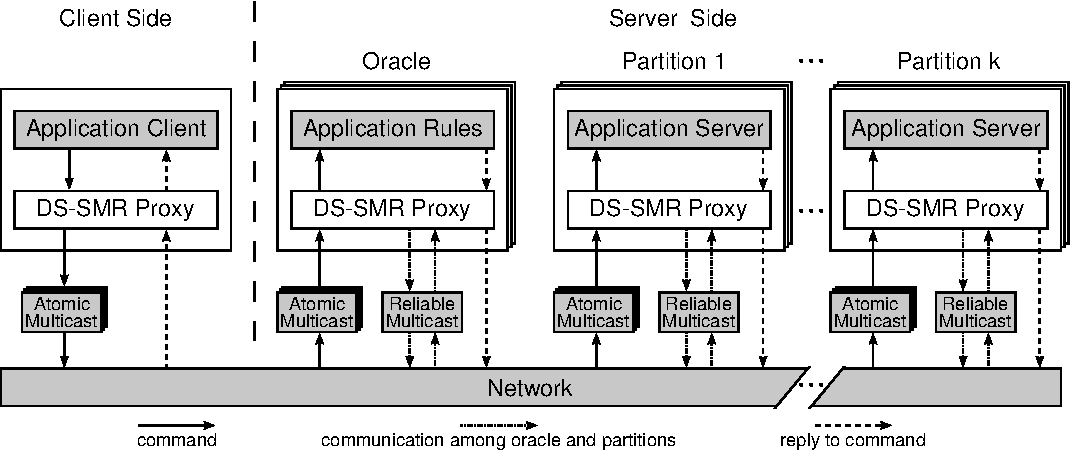
\includegraphics[width=0.8\linewidth]{figures/dssmr-arch}
\end{minipage}
\caption{The architecture of \dssmrlong{}.}
\label{fig:dssmr-arch}
\end{figure*}

